\documentclass{slide}

\usepackage{changepage}
\usepackage{tabto}
% \usepackage{pgfpages}
% \setbeameroption{show notes on second screen}

\title{Microservices Architecture}
\subtitle{Software Architecture}
\author{Richard Thomas}
\date{\week{10}}

\begin{document}

\maketitle

\point[Microservices]{Inspired by DDD}

\definition{Bounded Context}{Logical boundary of a domain where particular terms and rules apply consistently.}

\image[height=.97\textheight]{diagrams/bounded-context.png}

%\image[height=.96\textheight]{diagrams/microservices-arch.png}

\image[trim=39 50 22 39,clip,height=\textheight]{../../notes/microservices/diagrams/microservices-arch.png}
\note[itemize]{
    \item Basic structure of a microservices architecture.
    \item UIs are fairly monolithic to provide a rich interface.
    \item Fairly common to have multiple UIs, some of which use a different combination of services.
}

\image[trim=39 50 22 39,clip,height=\textheight]{../../notes/microservices/diagrams/microservices-ui2.png}
\note[itemize]{
    \item More like a purist microservices architecture, where each service development team builds the service's UI(s).
    \item Typically needs some coordinating activity in the UI.
    \item Can still have multiple UIs (e.g. web, mobile, ...).
}

\definition{Service Cohesion Principle}{Services are cohesive business processes. They are a bounded context.}

\definition{Service Independence Principle}{Services should not depend on the implementation of other services.}

\corollary{Low Coupling}{Services should have minimal coupling with other services.}

\corollary{No Reuse}{Services do not reuse components from other services, to avoid dependencies.}

\point[Choreography \& Orchestration]{
\begin{description}
    \item[Choreography] Similar to event-driven \highlight{broker}
    \item[Orchestration] Similar to event-driven \highlight{mediator}
\end{description}
}

\begin{frame}
    \begin{adjustwidth}{-10mm}{-10mm}
        \centering
        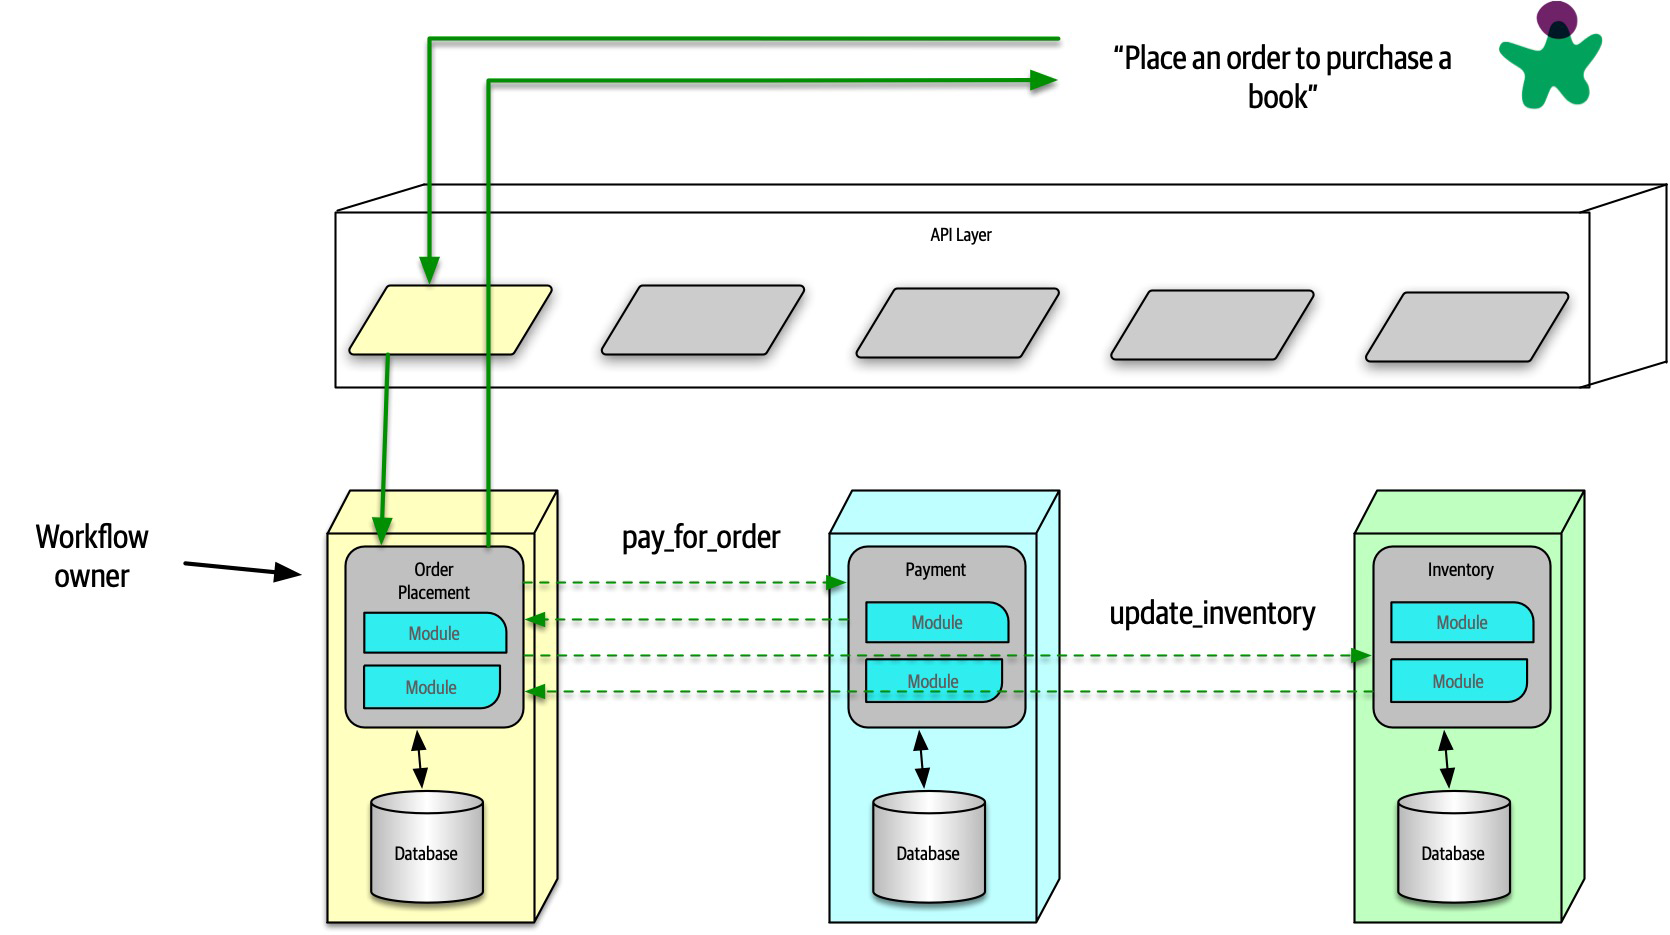
\includegraphics[width=0.96\paperwidth]{diagrams/choreography.png}
    \end{adjustwidth}
\end{frame}

\image[height=.98\textheight]{diagrams/orchestration.png}

\questionanswer{How bad is the coupling with choreography or orchestration?}
{For a very large system, very bad.}
\note{In 2017, Uber had over 1400 services ... consider how bad coupling would be with either approach.}

\image[trim=39 40 20 39,clip,height=\textheight]{../../notes/microservices/diagrams/microservices-queue.png}
\note[itemize]{
    \item Use the tried and true Observer pattern, with the event-driven architecture pattern.
    \item Services publish events indicating what they have been done.
    \item Services listen for events to decide what to coordinate system behaviour.
}

\image[trim=140 160 140 195,clip,height=\textheight]{diagrams/sahara-microservices-1-deploy.png}
\note[itemize]{
    \item Sahara eCommerce system as a simple microservices architecture, using event-driven messaging between services.
    \item Services publish events indicating what they have been done.
    \item Also an example of a multi-tenanted system built across in-house servers, AWS and OCI.
}

\questionanswer{Are \highlight{browsing} and \highlight{purchasing} separate contexts?}{
\begin{itemize}
    \item Are the a single business process or different processes?
    \item Do they share much or little data?
\end{itemize}
}
\note[itemize]{
    \item Probably different business processes, but possibly the same context.
    \item If separate services, browse needs to send an event for every change to the shopping cart, and purchase needs to listen for these.
    \item Possibly merge into one service, as one context.
}

\question{
\begin{itemize}
    \item What about \highlight{inventory management} and \highlight{browse}?
    \item How do they maintain a consistent product database?
\end{itemize}
}

\begin{frame}{Pros \& Cons}
    \vspace{1mm}
    {\LARGE
    \begin{description}
        \item[Modularity] \tabto{15em}
\includegraphics[width=8mm]{../../shared/images/thumbs-up.png}
        \item[Extensibility] \tabto{15em}
\includegraphics[width=8mm]{../../shared/images/thumbs-up.png}
        \item[Reliability] \tabto{15em}
\includegraphics[width=8mm]{../../shared/images/thumbs-up.png}
        \item[Interoperability] \tabto{15em}
\includegraphics[width=8mm]{../../shared/images/thumbs-up.png}
        \item[Scalability] \tabto{15em}
\includegraphics[width=8mm]{../../shared/images/thumbs-up.png}
        \item[Security] \tabto{15em}
\includegraphics[trim=57 145 70 85,clip,width=8mm]{../../shared/images/neutral.png}
        \item[Deployability] \tabto{15em}
\includegraphics[trim=22 19 22 12,clip,width=8mm]{../../shared/images/neutral.png}
        \item[Testability] \tabto{15em}
\includegraphics[trim=22 19 22 12,clip,width=8mm]{../../shared/images/neutral.png}
        \item[Simplicity] \tabto{15em}
\includegraphics[trim=22 19 22 12,clip,width=8mm]{../../shared/images/thumbs-down.png}
    \end{description}
    }
\end{frame}

\end{document}